%% LyX 2.0.2 created this file.  For more info, see http://www.lyx.org/.
%% Do not edit unless you really know what you are doing.
\documentclass[english]{article}
\usepackage{utopia}
\usepackage{helvet}
\usepackage{courier}
\renewcommand{\familydefault}{\rmdefault}
\usepackage[T1]{fontenc}
\usepackage[latin9]{inputenc}
\usepackage[a4paper]{geometry}
\geometry{verbose,tmargin=2cm,lmargin=2cm,footskip=2cm}
\setlength{\parskip}{\medskipamount}
\setlength{\parindent}{0pt}
\usepackage{refstyle}
\usepackage{graphicx}
\usepackage{setspace}

\makeatletter

%%%%%%%%%%%%%%%%%%%%%%%%%%%%%% LyX specific LaTeX commands.

\AtBeginDocument{\providecommand\subref[1]{\ref{sub:#1}}}
%% Special footnote code from the package 'stblftnt.sty'
%% Author: Robin Fairbairns -- Last revised Dec 13 1996
\let\SF@@footnote\footnote
\def\footnote{\ifx\protect\@typeset@protect
    \expandafter\SF@@footnote
  \else
    \expandafter\SF@gobble@opt
  \fi
}
\expandafter\def\csname SF@gobble@opt \endcsname{\@ifnextchar[%]
  \SF@gobble@twobracket
  \@gobble
}
\edef\SF@gobble@opt{\noexpand\protect
  \expandafter\noexpand\csname SF@gobble@opt \endcsname}
\def\SF@gobble@twobracket[#1]#2{}
\RS@ifundefined{subref}
  {\def\RSsubtxt{section~}\newref{sub}{name = \RSsubtxt}}
  {}
\RS@ifundefined{thmref}
  {\def\RSthmtxt{theorem~}\newref{thm}{name = \RSthmtxt}}
  {}
\RS@ifundefined{lemref}
  {\def\RSlemtxt{lemma~}\newref{lem}{name = \RSlemtxt}}
  {}


\AtBeginDocument{
  \def\labelitemii{\(\circ\)}
  \def\labelitemiii{\normalfont\bfseries{--}}
}

\makeatother

\usepackage{babel}
\begin{document}

\title{{\Huge CS26110 Assignment 1}}


\author{{\Large Samuel Jackson - slj11@aber.ac.uk}}

\maketitle

\section{Sliding Tile Puzzle}


\subsection{Node Representation}

The problem of representing each node in the sliding tile puzzle within
a search tree could be solved by using a fixed length array of size
7 where each element in the array represents a single tile in the
sliding puzzle. The array could either store a list of characters
of either B, R or space (representing the blue, red and empty slot
respectively). This representation would be useful when outputting
he resulting node to the user. Alternatively the problem could be
represented using a trit array (with values 0, 1 and 2) where each
trit represents a character in the array (or a space)\@. 

The reason why I believe an array to be a good choice for the representation
of a node is that regardless of what symbol is used to signify a red,
blue or space tile, the indices's of the array give a handle to the
tiles position in the grid. The indices's of the array can then be
used to swap the space with red and blue tiles. A tile's position
in the array can also be used to calculate whether it is close enough
to move into the empty space and calculate the cost of the move.


\subsection{Initial State Tree}

The diagram below shows all of the initial valid moves from the start
state of the sliding puzzle game. The cost of the moves are shown
alongside the line branching from the start state.

\begin{figure}[!tph]
\noindent \begin{centering}
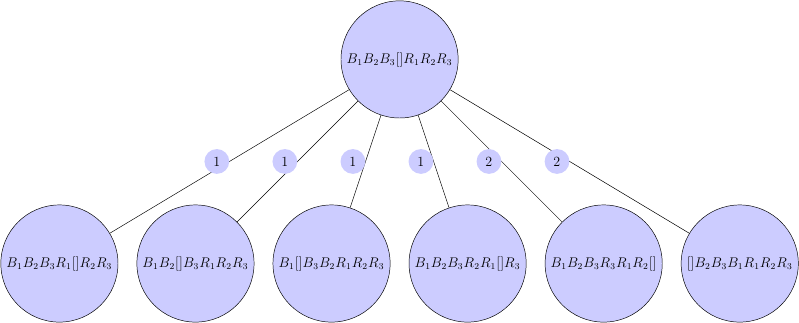
\includegraphics[scale=0.8]{graph}
\par\end{centering}

\caption{All possible moves from the start state, including the cost of the
moves.}
\end{figure}


\clearpage{}


\subsection{Uninformed Search Strategy}

\begin{singlespace}
\noindent An uninformed search strategy could be used to solve the
sliding puzzle providing that we have enough time and memory resources
to represent and traverse the tree of valid moves. Although it is
not specified by the rules of the game, it is obviously desirable
that whatever search strategy we adopt to solve this puzzle should
attempt to give us an optimal solution. It is also desirable that
the search strategy is a complete one, as we know from the rules of
the puzzle that there will always be more than one distinct solutions
to the sliding puzzle because the end placement of the space does
not matter.
\end{singlespace}

I would suggest that the best uninformed search technique for this
problem would be to use a uniform cost search to traverse the search
space. There are several reasons why this is a good choice for the
given problem. Firstly, uniform cost search takes into account the
path cost of each edge between nodes in the search space. This means
that the algorithm will try to take the lowest cost path between nodes
in order to find a solution. Because of this it will generally prefer
to take paths which do not involve a ``double jump'' to find the
solution. Secondly, uniform cost search is guaranteed to find a solution
which is both complete and optimal, so we are guaranteed to get the
shortest, lowest cost path from the initial configuration to the end
state.

Comparing this search strategy to other search techniques provides
further support for my proposed use of uniform cost search. Both depth-first
and depth-limited search techniques are not guaranteed to return an
optimal solution. Also, depth-limited search is not guaranteed to
return any solution at all, despite the fact that the search tree
will always contain a number of different solutions. Clearly these
options do not provide a viable solution to the given problem.

Other available search strategies include using a breadth-first search
or a bi-directional search. Uniform cost search is effectively just
a breadth-first search, except that uniform cost search considers
path weights and breadth-first search does not. If all of the path
weights were the same positive number then uniform cost search would
exactly mimic a breadth-first search. Therefore on average we will
get better performance out of a uniform cost search ($O(b^{1+C^{*}/\varepsilon})$
time where $C^{*}$ is the cost of the optimal solution), and in the
worst case its performance will equal that of a breadth-first search
($O(b^{d})$ time). Because of this, breadth-first search only guarantees
to find us the shallowest solution, but not necessarily the lowest
cost path to a solution.

A bi-directional search offers another option for consideration for
an uninformed search strategy. Bi-directional search could be used
to traverse both from the start configuration and at the same time
traverse backwards from one of the end states. However, immediately
there is a problem with this approach. Seeing as there are multiple
ways to successfully complete the puzzle, how do we decide which end
configuration to start from? One end configuration may yield a shorter
path compared with another configuration and is therefore more desirable.
Bi-directional search offers better time complexity compared with
a breadth-first search as it effectively cuts the number of nodes
that need to be expanded in half. However, it still does not consider
the weight on any of the edges. Because of this, uniform cost search
can potentially provide us with a better solution compared with a
bi-directional search.

One final search strategy that could be considered is the use of the
iterative deepening depth-first search. This will have a lower space
complexity than uniform cost search, but still exhibits much of the
same issues as a breadth-first search. Mainly that it does not make
any attempt to consider the weight of the edge between two nodes,
and therefore is not guaranteed to find the lowest cost solution,
although it will find a complete one.

In conclusion, I believe that a uniform cost search is the clear uninformed
search technique to be used to solve the sliding tile puzzle as it
offers us a complete and optimal solution in a reasonable time and
space complexity. However, traverse of the search space could be dramatically
improved through the use of a heuristic as discussed in the next section.


\subsection{Search Heuristic%
\footnote{This section of the document answers questions 1(d) and 1(e) of the
assignment together.%
}}

One potential heuristic that could be used to solve this problem would
be to take the current configuration of the sliding tile puzzle and
assign to each tile a weight according to how many of the opposing
coloured tile is currently on the wrong side of this tile. Each of
these weights could then be summed and divided by two to give us a
heuristic estimate of how far away the current configuration is from
the target configuration. The reason that it must be divided by two
is that each time two tiles swap, the weight on each tile will decrease
by one, leading total reduction of two. Summing the total cost of
the tiles without dividing by two to account for this will lead to
an overestimate and therefore render this heuristic inadmissible.
This heuristic allows us to quantify how many tiles are out of order
without caring about where specific tiles end up (as would be the
case if we use a distance heuristic such as the Manhattan heuristic). 

In this heuristic, all of the titles initially have a weight of three
assigned to them. This is because the start configuration has all
of the blue tiles to the left of the red tiles and all of the red
tiles to the right of the blue tiles. Hence, for each tile in the
initial configuration, each has all three of the opposing colour on
the ``wrong'' side and therefore its weight is three. As the tiles
are moved around, some of them will jump over one another. At this
point two of tiles are now closer to the solution than their counterparts
and their weights will be modified accordingly as they will now only
have two tiles on the wrong side of them. Weights of each title would
continue to be reduced as the algorithm progresses until eventually
all tiles are in the correct configuration and the weights on each
tile are zero. 

The following diagram visually outlines part of a branch in the search
space from the initial configuration where tiles might move and how
their weights are adjusted accordingly. In this diagram, the subscripts
of each of the tiles represent the current weight that tile has. Shown
next to the node is the sum of the weights (our heuristic estimate)
for that particular configuration.

\begin{figure}[!tph]
\noindent \begin{centering}
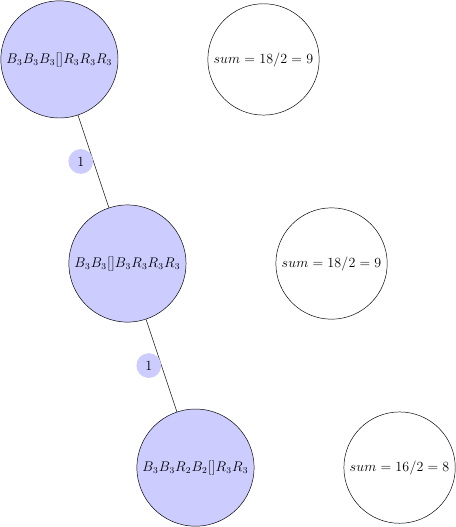
\includegraphics[scale=0.8]{graph_heuristic}
\par\end{centering}

\caption{An example of how the heuristic estimate changes as tiles are moved.}


\end{figure}


I believe this heuristic to be a a good choice for this problem for
several reasons. Initially, I considered that this puzzle presents
certain characteristics that are closely related n-puzzle problems.
Both problems involve sliding tiles around a fixed sized board and
they both have only one space which can be moved into at any one time.
Traditionally, one of the best heuristics used to solve a n-puzzle
is the Manhattan distance heuristic, which I initially thought could
be applied this problem. However there are several differences that
mean it would have produced sub optimal results.

The key difference between this puzzle and a n-puzzle is that tiles
in this puzzle can ``jump'' over two tiles at once, which incurs
a different path cost compared to jumping over a single tile or moving
into an open slot. Another key difference is that it does not matter
what order the tiles end up in, providing that all the blue tiles
end up on the opposite side of all the red tiles. This means that
the Manhattan distance is not exactly the best heuristic for this
problem, as I initially thought, because each tile does not have to
end up in a specific slot in the end configuration and therefore by
using the Manhattan distance heuristic it would incur more processing
than is actually required.

Subsequently while I believe that a Manhattan distance heuristic could
be of value to a search algorithm used to solve this problem, I decided
to scrap the idea in favor of a different technique that I have presented
here. My suggested heuristic will given an estimate of the total distance
left until we reach a solution, while not worrying about a tile moving
to a specific slot in the puzzle.

I would like to suggest that the heuristic function outlined in this
section is admissible, as it never overestimates the perfect solution
to the problem. At best it only ever gives a heuristic estimate that
is equal to the exact number of steps required to solve the problem.
Otherwise the heuristic will underestimate the distance required to
get from the initial configuration to a solution. This means that
the heuristic function will always lead us towards a complete and
optimal solution, rather than overestimating the path cost and returning
a sub optimal solution. We could also combine this heuristic with
an A{*} search to take account of the weights on the edges between
states. This would then find an optimal solution through the lowest
cost path to the solution while looking at a minimal number of states. 

However, there are a few downsides to this heuristic. One downside
is that it may underestimate the distance to the solution too much
during some configurations of the puzzle. In this case, the heuristic
offers little assistance to any search algorithm traversing the search
space and will look at more states than if the estimate were more
accurate. It may also be the case that certain moves do nothing to
lower the heuristic estimate, such sliding a tile into the empty slot
without jumping over anything. This would not lower the heuristic
estimate and therefore the heuristic would not provide any additional
information in this circumstance. However, despite these limitations,
the heuristic would still offer some assistance in guiding a search
algorithm towards an optimal goal state faster than an uninformed
search technique.


\section{Vehicle Grid Puzzle}


\subsection{Problem Definition}
\begin{enumerate}
\item \textbf{Initial State }- The initial state of this problem starts
with a set of $\ensuremath{n}$ vehicles arranged in an $\ensuremath{n\times n}$grid
so that they line up along the ``top'' side of the grid, with each
vehicle being in the first row of the grid and in the $\ensuremath{i}$-th
column.
\item \textbf{Goal State/Test }- We have reached the goal state if all of
the vehicles are in reverse order from there starting positions (i.e.
each tile is now at column $\ensuremath{n-i+1}$ where $\ensuremath{i}$
is the starting index of the agent) on the ``bottom'' ($\ensuremath{n^{th}}$)
row of the grid. We can test this by checking row $n$ of each column
to see if it contains vehicle $n-i+1$.
\item \textbf{Actions - }An agent in this state space can move one square
in any of the four directions defined in taxicab geometry providing
that the square is not occupied by another agent or that the given
direction takes the agent off of the grid. An agent may also chose
not to move at all from its current position during a given turn.
\item \textbf{Path Cost} - The puzzle description does not outline that
there is any specific cost associated with moving an agent to a new
square relative to there direction, so it can be assumed that every
move has an equal cost associated with it. Therefore each move an
agent makes can be defined as having a cost of 1. As it is undesirable
for each of the agents to not move, this will also have to incur a
cost of 1. Therefore the total path cost of a solution can be fully
quantified by how many total steps (in which each vehicle may or may
not move) it takes to get all vehicles to reach the goal state. 
\end{enumerate}

\subsection{Branching Factor}

The approximate branching factor of the vehicle grid problem is $5^{n}$.
This is because for each state in the search space, there will be
approximately five to the power of $n$ possible valid choices leading
to other valid states. This is because for every node in the search
space, each vehicle can potentially ``move'' in five different directions:
up, down, left, right and staying stationary. The reason why the branching
factor is raised to $n$ (the number of vehicles on the grid) is because
for every node, each vehicle on the grid will make one of its moves.
Therefore, we can choose one move for each of the vehicles on the
grid in any combination and so the product rule can be used to calculate
the total number of combinations. In the case of a grid of size five
where each vehicle can potentially move in up to five directions this
is approximately $5\times5\times5\times5\times5=5^{5}=3125$ possible
moves from each node.


\subsection{Minimum Number of Steps\label{sub:Minimum-number-of}}

The minimum number of steps required for one vehicle to move from
its current position at $(r_{i},c_{i})$, where $i$ is the index
of a column or row, can be expressed as the mathematical function:

\[
h_{i}(n)=|r_{i}-n|+|c_{i}-(n-i+1)|
\]


Which gets us the vehicle $i$'s Manhattan distance from it's current
position in the grid to its finishing position at $n-i+1$. This formula
works by getting the absolute difference between the vehicles current
row and the target row. It then sums this with the absolute difference
between the current column and the target column for this vehicle
($n-i+1$). As an example, lets say that a vehicle of index $3$ is
on an empty $5\times5$ grid at position $(3,4)$ then according to
the formula above, the distance it would have to travel to reach its
goal state would be a minimum of $3$ moves. Note that this formula
will work with any $n\times n$ grid; not just for a grid of size
five.


\subsection{Vehicle Grid Heuristic}

The function outlined in the preceding section could be used as part
of a heuristic function to help aid a search algorithm to solve the
vehicle grid problem. The underlying principle of function $h_{i}$
is that it calculates the Manhattan distance for the current vehicle
to the goal state. In other words, based on the current position of
the vehicle, it calculates how many steps, at minimum, need to be
taken for the vehicle to reach its destination square. A heuristic
function can use this to estimate the minimum number of moves required
to get all of the vehicles from their current state to the goal state.
To obtain a heuristic estimate, we simply apply the function outlined
in \subref{Minimum-number-of} to each of the vehicles in a given
state and then sum the results as shown by the following formula:

\[
{\scriptstyle {\displaystyle h(n)=\sum_{i=1}^{i=n}h_{i}(n)}}
\]


Where $h(n)$ is the heuristic cost estimate of moving all the vehicles
from there current state on the grid to there goal states. Of course,
this heuristic is not perfect, as it only takes into account how many
moves need to be taken by a vehicle to get to its goal state on an
empty grid. The Manhattan distance heuristic in no way accounts for
other vehicles getting in the way of the current vehicle's path and
therefore forcing it to either not move this step or to take a different
(sub optimal) direction. However, this feature does mean that the
heuristic is admissible as it will always be less than or equal to
the actual total distance required for a vehicle to reach its goal
state. Therefore the best search technique to use for this problem
would be to use an A{*} search that takes account of the total distance
traveled by each of the given vehicles for its path cost and uses
the heuristic function $h(n)$ in order to find a optimal route through
the search space.
\end{document}
